\documentclass[letterpaper, 12pt]{math}

\usepackage{graphicx}

\geometry{letterpaper, margin=0.5in}

\title{Intro to Computer Science Theory: Homework 2}
\author{Alvin Lin}
\date{August 2017 - December 2017}

\begin{document}

\maketitle

\subsection*{Problem 1}
Give FA state transition diagrams for the following languages. Be sure to label
the names of your states. Each language is over the alphabet \( \{a,b\} \),
and is defined as the set of all strings.
\begin{enumerate}
  \item that begin or end in \( aa \) in \( bb \).
    \begin{center}
      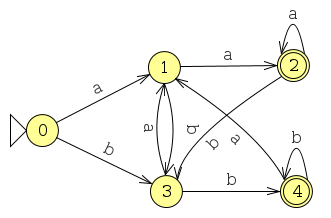
\includegraphics[width=8cm]{hw2_1_1.png}
    \end{center}
  \item that do not have \( aaa \) as a substring.
    \begin{center}
      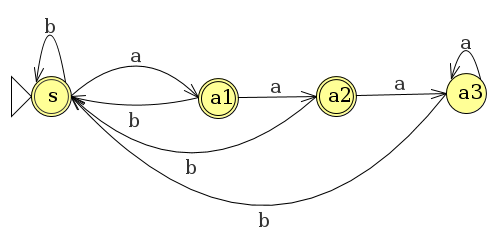
\includegraphics[width=10cm]{hw2_1_2.png}
    \end{center}
  \item that contain both \( aba \) and \( bab \) as substrings.
    \begin{center}
      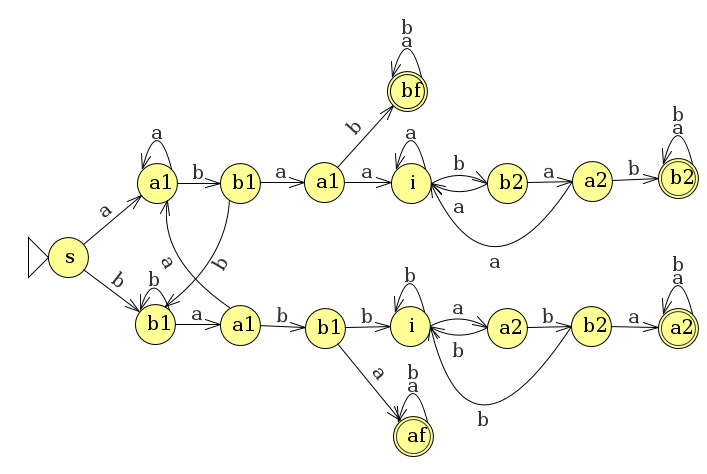
\includegraphics[width=15cm]{hw2_1_3.png}
    \end{center}
  \item whose length is a multiple of 5.
    \begin{center}
      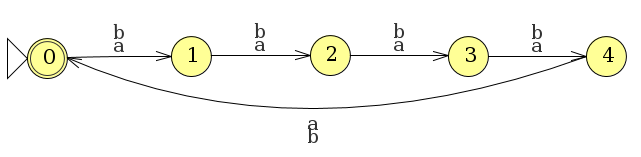
\includegraphics[width=12cm]{hw2_1_4.png}
    \end{center}
  \item where the number of \( a \)'s after the last \( b \) in the string is
    odd.
    \begin{center}
      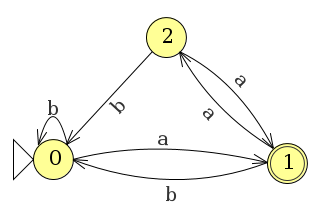
\includegraphics[width=8cm]{hw2_1_5.png}
    \end{center}
\end{enumerate}

\subsection*{Problem 2}
Provide formal definitions for 1, 4, and 5 above. Try to make them as concise
as possible.

\subsubsection*{Finite Automaton 1}
\( M = \{Q,\Sigma,\delta,0,\{2,4\}\} \) where:
\begin{itemize}
  \item \( Q = \{0,1,2,3,4\} \)
  \item \( \Sigma = \{a,b\} \)
  \item \( \delta: Q\times E\to Q \) is defined on \( (q,z)\in Q\times Z \) as:
    \[ \delta(q,x) = \begin{cases}
      1 & if\ (x = a) \wedge (q\in\{0,3,4\}) \\
      2 & if\ (x = a) \wedge (q\in\{1,2\})   \\
      3 & if\ (x = b) \wedge (q\in\{0,1,2\}) \\
      4 & if\ (x = b) \wedge (q\in\{3,4\})
    \end{cases} \]
\end{itemize}

\subsubsection*{Finite Automaton 4}
\( M = \{Q,\Sigma,\delta,0,\{0\}\} \) where:
\begin{itemize}
  \item \( Q = \{0,1,2,3,4\} \)
  \item \( \Sigma = \{a,b\} \)
  \item \( \delta: Q\times E\to Q \) is defined on \( (q,z)\in Q\times Z \) as:
    \[ \delta(q,x) = q+1 \]
\end{itemize}

\subsubsection*{Finite Automaton 5}
\( M = \{Q,\Sigma,\delta,0,\{1\}\} \) where:
\begin{itemize}
  \item \( Q = \{0,1,2\} \)
  \item \( \Sigma = \{a,b\} \)
  \item \( \delta: Q\times E\to Q \) is defined on \( (q,z)\in Q\times Z \) as:
    \[ \delta(q,x) = \begin{cases}
      0 & if\ (x = b) \\
      q+1 & if\ (x = a) \wedge (q \ne 2) \\
      1 & if\ (x = a) \wedge (q = 2)
    \end{cases} \]
\end{itemize}

\section*{Problem 3}

\begin{center}
  If you have any questions, comments, or concerns, please contact me at
  alvin@omgimanerd.tech
\end{center}

\end{document}
